\documentclass[11pt]{article}

\usepackage[a4paper,margin=20mm]{geometry}

\usepackage{amsmath,amssymb,array,booktabs,graphicx,float,longtable,hyperref,xcolor}

\definecolor{orange}{RGB}{190,95,0}

\hypersetup{colorlinks=true,urlcolor=blue}

\setlength{\parskip}{5pt}\setlength{\emergencystretch}{2em}

\title{Retained Hedging Models: Surface-Dynamics Audit}

\author{AI-agent implementation and diagnostic feedback}

\date{11 November 2026}

\begin{document}\maketitle

\section*{Executive summary}
\textbf{Purpose.} Assess the surface dynamics of retained rolling models on 44 April--May 2024 forecast origins, using one common log-IV grid and a PCA basis fixed before April. This is a model-law audit, not a rerun of hedging performance or a proof of no arbitrage.
\begin{itemize}
\item \textbf{DYSANOS: stationary backbone, weak observable dispersion.} All 88/88 distinct saved floating-volatility PCA--AR(1) backbones are stationary (maximum spectral radius 0.735). Nevertheless, pooled modeled log-IV-change variance is only 16.6\% of observed variance for ordinary PCA and 21.4\% for spot-orthogonal PCA. Stationarity is not the same as calibration.
\item \textbf{VolGAN: aggregate agreement hides conditional collapse.} Pooled modeled variance is 97.0\% of observed variance, but average within-origin forecast variance is only 0.025\%. A pooled variance ratio near one can therefore be misleading.
\item \textbf{Judge more than variance scale.} Compare covariance shape, spot leverage, forecast skill relative to persistence, and recursive behavior. A trace ratio near one is not an overall pass, and the conditional ratio need not equal one because its observed denominator is unconditional. GROMM-Q comparisons with historical P outcomes are descriptive, not P-calibration requirements.
\item \textbf{Tail conclusions remain preliminary.} Forty-four realized dates imply only 0.44 expected exceptions at a 1\% tail and 2.2 at a 5\% tail. Non-rejection cannot establish tail calibration. Stable AR coefficients and finite simulated paths do not prove non-explosion of the complete decoded model.
\item \textbf{Coverage at this report build.} Completed model--origin checks: surface forecasts 440/440; quote forecasts 440/440; recursive path tests 440/440. All requested origin-level diagnostics are complete; completion does not imply a model-quality pass.
\end{itemize}
\textbf{Interpretation.} These are diagnostics of retained implementations, including disclosed numerical guards and differing SANOS input smoothnesses, not a controlled architecture-only comparison. Black/orange/red colors use the explicit review tolerances in each table caption; they are not universal statistical acceptance criteria.
\clearpage

\section{Scope and headline findings}

The audit covers 44 origins from 1 April through 31 May 2024; the final one-session forecast settles on 3 June. Existing fits are retained unchanged. DYSANOS means our own saved floating-DLV PCA/AR(1) fits, not the latest external SANOS package. Results are diagnostics of retained legacy fits, not validation of the corrected hedge2 specification.

The observable reference is the retained public-candidate SANOS interpolation (smoothness 0.25), manifest \texttt{2add65d6\ldots}. Our DYSANOS coordinates instead came from the licensed smoothness-0.1 interpolation. These are not identical input pipelines; the comparison therefore measures retained-system behaviour, not architecture alone.

\textbf{Main distinction:} pooled covariance can look realistic even when a model has almost no conditional randomness. VolGAN is the clearest example. Persistence is measured using one pre-April observable PCA basis, never by concatenating rolling native factor scores. The DYSANOS stationarity assessment concerns only its floating-volatility PCA--AR(1) backbone; spot-level stationarity is neither required nor tested. All 44 fitted backbones in each DYSANOS variant admit a stationary distribution.

\begin{table}[H]\centering\small\setlength{\tabcolsep}{4pt}
\caption{Diagnostic coverage: dates evaluated out of the 44 requested April--May 2024 origins. Color rules: Black: all 44 requested origins evaluated. Orange: fewer than 44. No red coverage grade; coverage is not model quality. Missing graded entries are orange; other raw quantities are ungraded.}\label{tab:audit-coverage}
\begin{tabular}{@{}lrrrr@{}}
\toprule
Model & Requested dates & Surface dates & Quote dates & Path-test dates \\
\midrule
DYSANOS ordinary (16 factors) & 44 & \textcolor{black}{44} & \textcolor{black}{44} & \textcolor{black}{44} \\
DYSANOS spot-orthogonal (16 factors) & 44 & \textcolor{black}{44} & \textcolor{black}{44} & \textcolor{black}{44} \\
FuNVol & 44 & \textcolor{black}{44} & \textcolor{black}{44} & \textcolor{black}{44} \\
VolGAN PCA8 & 44 & \textcolor{black}{44} & \textcolor{black}{44} & \textcolor{black}{44} \\
AD-Seq-Vol & 44 & \textcolor{black}{44} & \textcolor{black}{44} & \textcolor{black}{44} \\
AD-Seq-Vol-FT & 44 & \textcolor{black}{44} & \textcolor{black}{44} & \textcolor{black}{44} \\
GROMM-P & 44 & \textcolor{black}{44} & \textcolor{black}{44} & \textcolor{black}{44} \\
GROMM-Q & 44 & \textcolor{black}{44} & \textcolor{black}{44} & \textcolor{black}{44} \\
DYSANOS ordinary (16 factors) (tail) & 44 & \textcolor{black}{44} & \textcolor{black}{44} & \textcolor{black}{44} \\
DYSANOS spot-orthogonal (16 factors) (tail) & 44 & \textcolor{black}{44} & \textcolor{black}{44} & \textcolor{black}{44} \\
\bottomrule\end{tabular}\end{table}

Table~\ref{tab:audit-coverage} is a coverage inventory, not a performance or pass/fail table. Surface dates count origins with evaluated next-day IV forecasts for covariance and tail diagnostics. Quote dates count origins with exact next-day contract matches for price-forecast scoring. Path-test dates count completed recursive floating-IV tests, including tests that produced no wholly valid decoded IV paths. Such failures contribute their actual invalid rates to Table~\ref{tab:recursive-stability}; they are not hidden as missing coverage. Each entry counts dates, not Monte Carlo paths; zero means no completed test, not a model-quality failure.

Covariance/tail availability follows retained next-surface arrays or newly sampled saved fits. The base-diffusion first next-IV artifact was absent: 512 new CPU scenarios were generated from its existing 1 April EMA checkpoint, with no retraining; its other 43 dates retain their 10,000-path forecasts. At the user's request, 22 additional May FT fits now continue the original April chain sequentially, using the unchanged selected one-epoch rolling update and causal 252-observation windows. Training completion is distinct from forecast-scenario availability in Table~\ref{tab:audit-coverage}. Quote forecasts can use retained price-return books independently of IV arrays. The previously missing 20 May quote join was a normalized-strike float32 round-trip identity bug, not absent quotes. The corrected join accepts a source cash strike only when it is the unique candidate within four float32 machine epsilons times the reconstructed cash-strike scale. Ambiguous and more distant contracts remain excluded; per-date maximum identity errors are retained.

Every model uses the same 32-path, 115-business-session protocol on the same 44 origins, with seed 20261111. Completed neural paths reuse their identical first 115 sessions; partial diffusion checkpoints preserve the original context and RNG state. Native models retain their different stochastic laws, not artificially identical generated prices. GROMM's final saved expiry is 125D and the observable grid extends to 10D, so 115 sessions is the common horizon without inventing expiries or long-end extrapolation. Its aged maturities are decoded by total-variance interpolation at fixed normalized strike, with a zero-maturity variance anchor (flat short-end IV). All models use their own generated history, never future observed states. Coverage counts only completed tests; queued work is not a pass.

\section{Traffic-light interpretation and origins of thresholds}

Black means within the stated review tolerance, orange means warning or insufficient evidence, and red means outside tolerance or a rejected diagnostic null. These are diagnostic-specific labels, not a proof of arbitrage-freedom and not a ranking of trading profitability. Counts, reference values and proper scores without a comparison baseline are shown neutrally. Missing evidence is orange, never a pass.

{\small\setlength{\tabcolsep}{3pt}\begin{longtable}{@{}>{\raggedright\arraybackslash}p{.25\linewidth}>{\raggedright\arraybackslash}p{.22\linewidth}>{\raggedright\arraybackslash}p{.25\linewidth}>{\raggedright\arraybackslash}p{.22\linewidth}@{}}
\caption{Retrospective traffic-light rules. Black: pass under the stated review tolerance; orange: warning or insufficient evidence; red: outside tolerance or a rejected diagnostic null. Missing evidence is orange. Boundaries are inclusive except where stated.}\label{tab:grading-rules}\\
\toprule Diagnostic & Pass (black) & Warn (orange) & Fail (red)\\\midrule\endfirsthead
\toprule Diagnostic & Pass (black) & Warn (orange) & Fail (red)\\\midrule\endhead
Covariance Frobenius error & at most 0.25 & above 0.25, at most 0.50 & above 0.50 \\
Variance trace ratio & 0.80 to 1.25 & 0.50 to 2.00, outside pass & outside 0.50 to 2.00 \\
Leading-share L1 error & at most 0.10 & above 0.10, at most 0.25 & above 0.25 \\
Subspace angle & at most 15 degrees & above 15, at most 30 degrees & above 30 degrees \\
Spot-correlation or IV-ACF error & at most 0.10 & above 0.10, at most 0.20 & above 0.20 \\
Forecast loss / persistence & at most 1.00 & above 1.00, at most 1.10 & above 1.10 \\
Reconstruction inside spread & at least 95\% & 80\% to below 95\% & below 80\% \\
Reconstruction mean outside distance & at most 0.25 spreads & above 0.25, at most 1 spread & above 1 spread \\
Reconstruction q95 outside distance & at most 1 spread & above 1, at most 2 spreads & above 2 spreads \\
May/April relative-skill deterioration & at most 1.10 & above 1.10, at most 1.25 & above 1.25 \\
Exact-binomial tail coverage & p at least .05 and 10 expected exceptions & p at least .01 but not pass & p below .01 \\
PCA AR spectral radius & below .99 & .99 to below 1 & at least 1 \\
Invalid decoded paths & zero & above zero, at most 1\% & above 1\% \\
Surfaces with IV above 300\% & zero & above zero, at most 0.1\% & above 0.1\% \\
Diagnostic coverage & all requested dates & partial coverage or not run & not a model-quality failure \\
\bottomrule\end{longtable}}

Only the AR boundary $\rho(A)=1$ comes from the mathematical stationarity condition. The nearby .99 warning is a practical slow-reversion flag: $\log(1/2)/\log(.99)\simeq69$ business sessions. Tail cutoffs .05 and .01 are conventional pointwise type-I error levels for the exact binomial coverage test, not Gaussian standard-error approximations. Fewer than ten expected exceptions prevents a black tail result even if the null is not rejected. An IV-ACF comparison with fewer than 30 observed lag pairs likewise cannot receive black.

All remaining boundaries are explicit, round-number engineering tolerances introduced for this retrospective review, not confidence bounds, published universal standards, or thresholds selected on a separate validation set. Frobenius bounds permit 25\%/50\% norm error; trace bounds permit a factor 1.25/two mismatch; eigen-share bounds permit 10/25 percentage points of summed error; correlation bounds permit .10/.20 absolute error. The spread and forecast tolerances express stated reconstruction goals and allowed deterioration against a simple persistence forecast. They were not used to choose or retrain the models and should be sensitivity-tested before any production acceptance decision.

Next-day forecast in-spread rates and mean outside distances are not graded as reconstruction: a correct conditional expectation need not lie in a narrow realized next-day spread. Price-prediction grading instead compares MAE with the same contracts' origin observed midpoints carried by the origin-only one-day discount factor. Log-IV forecast RMSE is compared with the no-change IV forecast. A ratio at most one means no deterioration; up to 1.10 is the explicit 10\% warning band. May/April deterioration compares these persistence-normalized log-IV losses, reducing confusion with changing market volatility. Pinball and joint VaR--ES scores are proper-score comparisons, not zero-centered tests; tail colors refer to coverage, not their raw score magnitudes.

Colors on conditional covariance/trace are descriptive dispersion screens against realized total covariance, not formal conditional-covariance tests; between-origin predicted means can explain a difference. Tail p-values and colors are pointwise and exploratory; no across-model multiplicity correction is claimed. Historical-P comparisons for GROMM-Q are descriptive, not a demand that a Q generator reproduce P outcomes. The complete numeric rules are saved in \texttt{TRAFFIC\_LIGHT\_RULES.json}.

\section{Surface covariance and spot leverage}

The common grid has business-day tenors $(1,2,3,4,5,7,10)$ and NMS $(-1.5,-1,-0.5,0,0.5,1,1.5)$, giving 49 equally weighted log-IV coordinates. The central common domain avoids comparing different native grids or extreme-wing inversion conventions. All retained reference nodes in this common domain have interior IVs; the broader native reference grid does contain repaired wing nodes. This is not a test of the omitted wings. Native grids remain unchanged.

The fixed three-PC basis uses 252 exact one-session training transitions with endpoints 2023-02-21--2024-03-28, strictly before April. These are eligible retained transitions, not an assertion of 252 consecutive calendar sessions. Their variance shares are 78.19, 10.80, 3.83 percent (total 92.81 percent). No whitening or per-model refitting of this audit basis is used.

Let $x_t$ be the common log-IV vector, $U$ the fixed basis, $\Delta x_{t+1}=x_{t+1}-x_t$, $m_t=E_t[\Delta x_{t+1}]$ and $C_t=\operatorname{Cov}_t(\Delta x_{t+1})$. We compare both $\bar C$ and $\bar C+\widehat{\operatorname{Cov}}_t(m_t)$ with the sample covariance of observed changes. The latter retains between-origin variation in conditional means; it must not be mistaken for conditional shock dispersion. Across-origin covariance uses denominator $n-1$; the displayed sum is the fixed-design, sample-covariance convention. Monte Carlo forecast covariance uses the sample convention, whereas exact enumeration of the 252-atom DYSANOS law uses its population denominator 252.

\[E_F=\frac{\|\Sigma_{\rm model}-\Sigma_{\rm data}\|_F}{\|\Sigma_{\rm data}\|_F}.\]

\begin{table}[H]\centering\small\setlength{\tabcolsep}{4pt}
\caption{Surface covariance errors and variance ratios on each model's available dates. Color rules: Frobenius error: black at most 0.25, orange above 0.25 through 0.50, red above 0.50. Trace ratio: black 0.80--1.25; orange 0.50--2.00 outside that band; red outside 0.50--2.00. These are descriptive review tolerances, not statistical acceptance tests. Missing graded entries are orange; other raw quantities are ungraded.}\label{tab:surface-covariance}
\begin{tabular}{@{}lrrrrr@{}}
\toprule
Model & Days & Frob. cond. & Frob. pooled & Trace cond. & Trace pooled \\
\midrule
DYSANOS ordinary (16 factors) & 44 & \textcolor{red}{0.914} & \textcolor{red}{0.821} & \textcolor{red}{0.080} & \textcolor{red}{0.166} \\
DYSANOS spot-orthogonal (16 factors) & 44 & \textcolor{red}{0.839} & \textcolor{red}{0.775} & \textcolor{red}{0.155} & \textcolor{red}{0.214} \\
FuNVol & 44 & \textcolor{red}{0.602} & \textcolor{red}{0.580} & \textcolor{red}{0.397} & \textcolor{red}{0.495} \\
VolGAN PCA8 & 44 & \textcolor{red}{1.000} & \textcolor{orange}{0.283} & \textcolor{red}{0.000251} & \textcolor{black}{0.970} \\
AD-Seq-Vol & 44 & \textcolor{red}{0.665} & \textcolor{red}{0.786} & \textcolor{red}{0.374} & \textcolor{orange}{1.542} \\
AD-Seq-Vol-FT & 44 & \textcolor{red}{0.740} & \textcolor{red}{0.697} & \textcolor{red}{0.302} & \textcolor{orange}{1.455} \\
GROMM-P & 44 & \textcolor{orange}{0.398} & \textcolor{orange}{0.334} & \textcolor{orange}{0.796} & \textcolor{orange}{1.268} \\
GROMM-Q & 44 & \textcolor{orange}{0.410} & \textcolor{orange}{0.280} & \textcolor{orange}{0.763} & \textcolor{black}{1.205} \\
DYSANOS ordinary (16 factors) (tail) & 44 & \textcolor{red}{0.914} & \textcolor{red}{0.820} & \textcolor{red}{0.080} & \textcolor{red}{0.166} \\
DYSANOS spot-orthogonal (16 factors) (tail) & 44 & \textcolor{red}{0.839} & \textcolor{red}{0.776} & \textcolor{red}{0.154} & \textcolor{red}{0.214} \\
\bottomrule\end{tabular}\end{table}

In Table~\ref{tab:surface-covariance}, the two Frobenius columns measure relative covariance-matrix error (zero is exact agreement); the two trace columns divide model by observed total log-IV-change variance (one is scale agreement). Figure~\ref{fig:surface-variance} plots those same trace columns. Its conditional bar uses the average within-origin forecast covariance; its pooled bar additionally includes between-origin forecast-mean variation. The color bands in the table caption are retrospective engineering review tolerances, not precommitted statistical pass/fail criteria. In particular, the conditional ratio need not equal one because the observed denominator is unconditional.

Table~\ref{tab:surface-covariance} uses each model's available dates. Table~\ref{tab:matched-covariance} restricts every model to the same 44 common origins (2024-04-01--2024-05-31). The PCA basis remains unchanged.

\begin{table}[H]\centering\small\setlength{\tabcolsep}{4pt}
\caption{Surface covariance comparison restricted to dates available for every model. Color rules: Frobenius error: black at most 0.25, orange above 0.25 through 0.50, red above 0.50. Trace ratio: black 0.80--1.25; orange 0.50--2.00 outside that band; red outside 0.50--2.00. These are descriptive review tolerances, not statistical acceptance tests. Missing graded entries are orange; other raw quantities are ungraded.}\label{tab:matched-covariance}
\begin{tabular}{@{}lrrrr@{}}
\toprule
Model & Matched days & Frob. pooled & Trace cond. & Trace pooled \\
\midrule
DYSANOS ordinary (16 factors) & 44 & \textcolor{red}{0.821} & \textcolor{red}{0.080} & \textcolor{red}{0.166} \\
DYSANOS spot-orthogonal (16 factors) & 44 & \textcolor{red}{0.775} & \textcolor{red}{0.155} & \textcolor{red}{0.214} \\
FuNVol & 44 & \textcolor{red}{0.580} & \textcolor{red}{0.397} & \textcolor{red}{0.495} \\
VolGAN PCA8 & 44 & \textcolor{orange}{0.283} & \textcolor{red}{0.000251} & \textcolor{black}{0.970} \\
AD-Seq-Vol & 44 & \textcolor{red}{0.786} & \textcolor{red}{0.374} & \textcolor{orange}{1.542} \\
AD-Seq-Vol-FT & 44 & \textcolor{red}{0.697} & \textcolor{red}{0.302} & \textcolor{orange}{1.455} \\
GROMM-P & 44 & \textcolor{orange}{0.334} & \textcolor{orange}{0.796} & \textcolor{orange}{1.268} \\
GROMM-Q & 44 & \textcolor{orange}{0.280} & \textcolor{orange}{0.763} & \textcolor{black}{1.205} \\
DYSANOS ordinary (16 factors) (tail) & 44 & \textcolor{red}{0.820} & \textcolor{red}{0.080} & \textcolor{red}{0.166} \\
DYSANOS spot-orthogonal (16 factors) (tail) & 44 & \textcolor{red}{0.776} & \textcolor{red}{0.154} & \textcolor{red}{0.214} \\
\bottomrule\end{tabular}\end{table}

\begin{figure}[H]\centering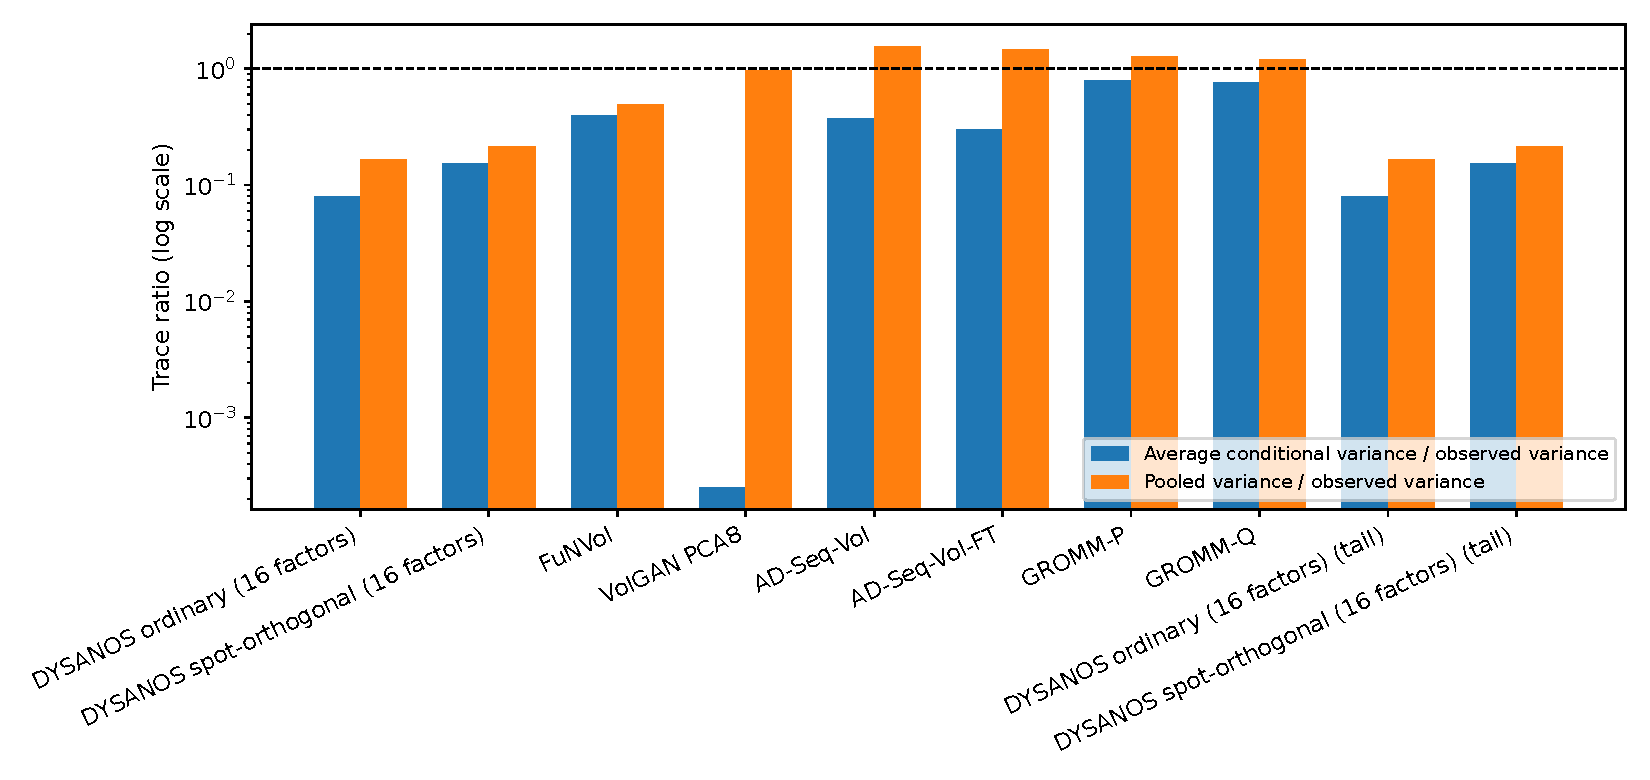
\includegraphics[width=\linewidth]{covariance.pdf}\caption{Conditional and pooled surface-variance ratios. The logarithmic scale makes underdispersion visible rather than hiding it behind changing forecast means.}\label{fig:surface-variance}\end{figure}

\subsection{Why native PCA coverage need not preserve IV variance}

The retained DYSANOS PCs minimize Euclidean reconstruction error in 1809 native log-DLV/forward-vol coordinates, not in option prices or log implied volatilities. Locally, if $J$ is the pricing/IV decoder Jacobian, the observable covariance is $J\Sigma_uJ'$. A PCA truncation that retains much of $\operatorname{tr}(\Sigma_u)$ need not retain much of $\operatorname{tr}(J\Sigma_uJ')$. Drift-adjusting the retained factors for AR fitting can further reduce innovation variance. Floors and nonlinear decoder guards also affect this mapping. Therefore a native coverage percentage is not an observable-variance guarantee.

\begin{table}[H]\centering\small\setlength{\tabcolsep}{4pt}
\caption{Same-shock variance reconciliation. Each origin uses the same 252 trailing centered native changes and current decoder. Percentages divide by the full centered-native-shock comparator: native energy for the first numeric column, decoded log-IV variance for the others. No shocks are inflated; the comparator is an ablation, not a fitted full-rank alternative. Original decoder guards remain active and their counts are retained. Color rules: Black: ungraded diagnostic quantities. Orange and red grades are not assigned; this ablation is not a calibration pass/fail test. Missing graded entries are orange; other raw quantities are ungraded.}\label{tab:variance-reconciliation}
\begin{tabular}{@{}lrrrr@{}}
\toprule
Model & Origin & Native retained \% & PCA IV \% & AR innovation IV \% \\
\midrule
DYSANOS ordinary (16 factors) & 2024-04-01 & 82.868 & 21.410 & 12.897 \\
DYSANOS ordinary (16 factors) & 2024-04-30 & 83.970 & 33.061 & 18.091 \\
DYSANOS ordinary (16 factors) & 2024-05-31 & 84.182 & 27.966 & 16.625 \\
DYSANOS spot-orthogonal (16 factors) & 2024-04-01 & 83.026 & 35.556 & 28.503 \\
DYSANOS spot-orthogonal (16 factors) & 2024-04-30 & 84.124 & 46.996 & 34.264 \\
DYSANOS spot-orthogonal (16 factors) & 2024-05-31 & 84.325 & 40.326 & 31.283 \\
\bottomrule\end{tabular}\end{table}

\subsection{Controlled eight-versus-sixteen-factor DYSANOS comparison}

Only the retained rank changes. Both variants use the same 44 origins, 252 exact causal training transitions, empirical paired spot innovations, native states, decoder guards and vector cdxcore IV inversion. Each new rolling basis is aligned with its preceding origin; March 28 supplies a causal alignment seed before scoring starts. The old eight-dimensional subspace is verified to lie inside the new sixteen-dimensional span at every origin. No shock inflation or tail multiplier is introduced. The separate recursive tests retain the common 32-path, 115-session protocol. This does not resolve the source/reference smoothness difference or change the native density fit.

\begin{table}[H]\centering\small\setlength{\tabcolsep}{4pt}
\caption{Controlled rank comparison on all 44 origins. Native coverage is averaged across origins; decoded covariance is compared against the unchanged observable reference. Counts, native coverage and covariance scale are distinct quantities. Color rules: Frobenius error: black at most 0.25, orange above 0.25 through 0.50, red above 0.50. Trace ratio: black 0.80--1.25; orange 0.50--2.00 outside that band; red outside 0.50--2.00. These are descriptive review tolerances, not statistical acceptance tests. AR spectral radius: black below 0.99, orange from 0.99 to below 1, red at least 1. Native coverage and counts are ungraded. Missing graded entries are orange; other raw quantities are ungraded.}\label{tab:rank-comparison}
\begin{tabular}{@{}lrrrrrr@{}}
\toprule
Variant / rank & Days & Native \% & Trace cond. & Trace pooled & Frob. pooled & Max radius \\
\midrule
Ordinary / 8 & 44 & 70.598 & \textcolor{red}{0.037} & \textcolor{red}{0.059} & \textcolor{red}{0.939} & \textcolor{black}{0.699} \\
Spot-orthogonal / 8 & 44 & 70.770 & \textcolor{red}{0.132} & \textcolor{red}{0.152} & \textcolor{red}{0.843} & \textcolor{black}{0.695} \\
Ordinary / 16 & 44 & 83.773 & \textcolor{red}{0.080} & \textcolor{red}{0.166} & \textcolor{red}{0.821} & \textcolor{black}{0.735} \\
Spot-orthogonal / 16 & 44 & 83.862 & \textcolor{red}{0.155} & \textcolor{red}{0.214} & \textcolor{red}{0.775} & \textcolor{black}{0.730} \\
\bottomrule\end{tabular}\end{table}

\begin{table}[H]\centering\small\setlength{\tabcolsep}{4pt}
\caption{Eight- and sixteen-factor same-shock ablations. Percentages use the same full native-shock comparator at each origin. Decoder guards remain active, so this is not an attribution to linear PCA alone. Color rules: Black: ungraded same-shock ablation quantities. Orange and red grades are not assigned; variance retention is not a calibration pass/fail test. Missing graded entries are orange; other raw quantities are ungraded.}\label{tab:rank-reconciliation}
\begin{tabular}{@{}lrrrr@{}}
\toprule
Variant / rank & Origin & Native retained \% & PCA IV \% & AR innovation IV \% \\
\midrule
Ordinary / 8 & 2024-04-01 & 68.928 & 7.536 & 4.880 \\
Ordinary / 8 & 2024-04-30 & 71.036 & 14.034 & 8.493 \\
Ordinary / 8 & 2024-05-31 & 71.392 & 14.754 & 9.047 \\
Ordinary / 16 & 2024-04-01 & 82.868 & 21.410 & 12.897 \\
Ordinary / 16 & 2024-04-30 & 83.970 & 33.061 & 18.091 \\
Ordinary / 16 & 2024-05-31 & 84.182 & 27.966 & 16.625 \\
Spot-orthogonal / 8 & 2024-04-01 & 69.203 & 26.962 & 23.991 \\
Spot-orthogonal / 8 & 2024-04-30 & 71.334 & 36.093 & 29.755 \\
Spot-orthogonal / 8 & 2024-05-31 & 71.667 & 32.473 & 26.499 \\
Spot-orthogonal / 16 & 2024-04-01 & 83.026 & 35.556 & 28.503 \\
Spot-orthogonal / 16 & 2024-04-30 & 84.124 & 46.996 & 34.264 \\
Spot-orthogonal / 16 & 2024-05-31 & 84.325 & 40.326 & 31.283 \\
\bottomrule\end{tabular}\end{table}

Full rank-comparison results, including PC1 tail counts, recursive invalid/extreme rates and decoder clipping counts, are retained in \texttt{rank\_comparison.json}. Native energy retention and a stable AR matrix do not by themselves establish observable covariance calibration.

Leading eigenvalue shares use the full covariance trace as denominator. Principal angles compare the leading three-dimensional subspaces of the full observable covariance; the table gives the maximum angle in degrees. The full machine-readable summary also contains the three-PC projected covariance comparison. Using three dimensions for a three-dimensional projected subspace angle would be vacuous, so only the full-space angles are interpreted.

\begin{table}[H]\centering\small\setlength{\tabcolsep}{4pt}
\caption{Log-IV forecast errors and leading covariance-subspace agreement. Color rules: RMSE: black at most the persistence RMSE, orange above persistence through 1.10 times persistence, red above 1.10 times. Maximum angle: black at most 15 degrees, orange above 15 through 30, red above 30. Eigen-share L1 error: black at most 0.10, orange above 0.10 through 0.25, red above 0.25. Missing graded entries are orange; other raw quantities are ungraded.}\label{tab:forecast-subspace}
\begin{tabular}{@{}lrrrr@{}}
\toprule
Model & Forecast RMSE & Persistence RMSE & Max angle & Share L1 error \\
\midrule
DYSANOS ordinary (16 factors) & \textcolor{black}{0.174} & 0.190 & \textcolor{red}{79.259} & \textcolor{orange}{0.151} \\
DYSANOS spot-orthogonal (16 factors) & \textcolor{black}{0.176} & 0.190 & \textcolor{red}{61.570} & \textcolor{orange}{0.127} \\
FuNVol & \textcolor{black}{0.183} & 0.190 & \textcolor{red}{48.536} & \textcolor{orange}{0.134} \\
VolGAN PCA8 & \textcolor{red}{0.215} & 0.190 & \textcolor{red}{48.630} & \textcolor{orange}{0.130} \\
AD-Seq-Vol & \textcolor{red}{0.237} & 0.190 & \textcolor{red}{51.960} & \textcolor{black}{0.096} \\
AD-Seq-Vol-FT & \textcolor{red}{0.266} & 0.190 & \textcolor{red}{52.164} & \textcolor{black}{0.077} \\
GROMM-P & \textcolor{black}{0.120} & 0.190 & \textcolor{red}{85.623} & \textcolor{orange}{0.102} \\
GROMM-Q & \textcolor{black}{0.125} & 0.190 & \textcolor{red}{85.754} & \textcolor{orange}{0.111} \\
DYSANOS ordinary (16 factors) (tail) & \textcolor{black}{0.174} & 0.190 & \textcolor{red}{72.909} & \textcolor{orange}{0.154} \\
DYSANOS spot-orthogonal (16 factors) (tail) & \textcolor{black}{0.176} & 0.190 & \textcolor{red}{58.317} & \textcolor{orange}{0.128} \\
\bottomrule\end{tabular}\end{table}

RMSE is in log-IV units over scored dates and all 49 cells. Persistence predicts no surface change. RMSE values concern raw model forecasts, not the artificial demeaning used by some hedge optimizers.

Spot leverage is $\operatorname{Corr}(r_{t+1},U_j^\top\Delta x_{t+1})$, where $r$ is the one-session forward-normalized log return. Signs are fixed by the training basis. Model values below use pooled joint moments; per-component absolute errors are in the JSON. A native DLV loading is not substituted for this observable correlation.

\begin{table}[H]\centering\small\setlength{\tabcolsep}{4pt}
\caption{Pooled correlations between spot returns and fixed-basis observable PC changes. Color rules: Absolute correlation error versus the observed reference: black at most 0.10, orange above 0.10 through 0.20, red above 0.20. Reference correlations and counts are neutral. Missing graded entries are orange; other raw quantities are ungraded.}\label{tab:spot-leverage}
\begin{tabular}{@{}lrrrr@{}}
\toprule
Model & Days & Spot/PC1 & Spot/PC2 & Spot/PC3 \\
\midrule
Observed reference & 44 & -0.680 & 0.157 & -0.008 \\
DYSANOS ordinary (16 factors) & 44 & \textcolor{red}{-0.149} & \textcolor{orange}{0.035} & \textcolor{black}{0.029} \\
DYSANOS spot-orthogonal (16 factors) & 44 & \textcolor{black}{-0.694} & \textcolor{red}{0.729} & \textcolor{red}{0.568} \\
FuNVol & 44 & \textcolor{black}{-0.711} & \textcolor{red}{0.457} & \textcolor{red}{0.232} \\
VolGAN PCA8 & 44 & \textcolor{red}{-0.451} & \textcolor{orange}{0.338} & \textcolor{red}{0.534} \\
AD-Seq-Vol & 44 & \textcolor{red}{-0.269} & \textcolor{orange}{0.318} & \textcolor{red}{0.263} \\
AD-Seq-Vol-FT & 44 & \textcolor{red}{-0.340} & \textcolor{red}{0.436} & \textcolor{red}{0.311} \\
GROMM-P & 44 & \textcolor{red}{-0.250} & \textcolor{black}{0.157} & \textcolor{black}{0.061} \\
GROMM-Q & 44 & \textcolor{red}{-0.214} & \textcolor{black}{0.149} & \textcolor{black}{0.076} \\
DYSANOS ordinary (16 factors) (tail) & 44 & \textcolor{red}{-0.147} & \textcolor{orange}{0.046} & \textcolor{black}{0.052} \\
DYSANOS spot-orthogonal (16 factors) (tail) & 44 & \textcolor{black}{-0.693} & \textcolor{red}{0.740} & \textcolor{red}{0.566} \\
\bottomrule\end{tabular}\end{table}

The JSON additionally separates correlations from the average conditional joint covariance and correlations of realized forecast residuals (observed changes minus each model's predicted means). This prevents between-origin mean variation from being mistaken for conditional spot leverage.

\section{Bid--ask fit and next-day prediction}

For quoted bid $b$, ask $a$ and predicted price $p$, outside distance is $d=\max(b-p,p-a,0)/(a-b)$. We report the in-spread share, mean and 95th percentile of $d$, and cash-price MAE. Crossed/zero-width/nonfinite inputs are excluded with counts. Quotes are licensed observed bid/ask, not fabricated spreads around fitted prices.

\begin{table}[H]\centering\small\setlength{\tabcolsep}{4pt}
\caption{Same-day quoted-spread reconstruction and next-day conditional-mean price prediction. Color rules: Same-day in-spread share: black at least 95\%, orange 80\% to below 95\%, red below 80\%. Forecast MAE / same-contract persistence MAE: black at most 1.00, orange above 1.00 through 1.10, red above 1.10. Other forecast statistics are ungraded; next-day in-spread share is not a reconstruction test. Missing graded entries are orange; other raw quantities are ungraded.}\label{tab:bidask-fit}
\begin{tabular}{@{}lrrrrrr@{}}
\toprule
Model & Recon. in & Pred. N & Pred. in & Mean distance & MAE / spot & MAE ratio \\
\midrule
DYSANOS ordinary (16 factors) & \textcolor{red}{0.744} & 44 & 0.013 & 36.830 & 0.002 & \textcolor{orange}{1.009} \\
DYSANOS spot-orthogonal (16 factors) & \textcolor{red}{0.744} & 44 & 0.010 & 37.309 & 0.002 & \textcolor{orange}{1.011} \\
FuNVol & \textcolor{orange}{--} & 44 & 0.013 & 43.205 & 0.002 & \textcolor{orange}{1.047} \\
VolGAN PCA8 & \textcolor{orange}{--} & 44 & 0.006 & 139.538 & 0.005 & \textcolor{red}{2.785} \\
AD-Seq-Vol & \textcolor{orange}{--} & 44 & 0.009 & 72.848 & 0.002 & \textcolor{red}{1.331} \\
AD-Seq-Vol-FT & \textcolor{orange}{--} & 44 & 0.007 & 69.679 & 0.002 & \textcolor{red}{1.284} \\
GROMM-P & \textcolor{orange}{0.928} & 44 & 0.009 & 43.425 & 0.002 & \textcolor{orange}{1.009} \\
GROMM-Q & \textcolor{orange}{0.928} & 44 & 0.009 & 41.915 & 0.002 & \textcolor{black}{0.995} \\
DYSANOS ordinary (16 factors) (tail) & \textcolor{red}{0.744} & 44 & 0.012 & 36.714 & 0.002 & \textcolor{orange}{1.010} \\
DYSANOS spot-orthogonal (16 factors) (tail) & \textcolor{red}{0.744} & 44 & 0.011 & 37.114 & 0.002 & \textcolor{orange}{1.011} \\
\bottomrule\end{tabular}\end{table}

Reconstruction uses all available quoted sides with origin tenors 1--10D and $|\mathrm{NMS}|\le1.5$ for DYSANOS and GROMM. Conditional IV generators do not have an independently fitted same-day observable decoder in this audit: their reconstruction is n/a, not perfect by copying their conditioning input. GROMM's stored 252-transition fit percentages are not substituted for today's measured quoted reconstruction.

Next-day prediction uses surviving OTM hedge-book contracts with origin tenors 2--5D and $|\mathrm{NMS}|\le1.5$, matched at their exact cash strike, expiry and settlement type. The expected raw scenario price is compared with tomorrow's observed spread. Financing/carry is fixed from the origin; tomorrow's spot/forward curve is not inserted into the forecast. Expiring 1D contracts are settlements, not next-day quotes. This is a limited retained-book forecast population, not every model-grid contract. Population, matched and excluded counts and moneyness-bucket scores are retained per date. Reconstruction and forecast columns have different populations and should not be compared as like-for-like fit rates.

A correct stochastic model need not put its conditional-mean forecast inside a narrow realized next-day spread. The forecast in-spread rate is a prediction diagnostic, not an arbitrage criterion. Quote aggregates give equal weight to dates, not to the number of contracts on each date. All daily counts, mean and 95th-percentile outside distances, price MAEs and buckets are retained in the CSV/JSON outputs.

\texttt{iv\_rmse\_buckets.csv} separately reports both log-IV RMSE and annual-IV RMSE for the explicitly defined point forecast $\hat\sigma_{t+1}=\exp(x_t+m_t)$, anchored to the common observed origin surface. This is a geometric-IV point forecast, not $E_t[\sigma_{t+1}]$ and not IV obtained by inverting a mean option price. Errors are bucketed by expiry and NMS. No realized forward is used to manufacture an IV from a potentially non-arbitrage-bounded mean price.

\section{Out-of-sample window stability}

Every available saved origin is scored. Monthly RMS errors are separated by April and May; no six-month evaluation is claimed. Both monthly and 21-origin rolling RMSE take the square root after averaging squared daily RMSE, consistent with the full-window metric. Rolling deterioration subtracts the first 21-origin value. A 63-session deterioration estimate is unavailable. These overlapping summaries are descriptive, not independent replications. Forecast horizon (one session), surface maturity (1--10 sessions) and evaluation-window length (44 origins) remain separate.

\begin{table}[H]\centering\small\setlength{\tabcolsep}{4pt}
\caption{Monthly next-day log-IV forecast RMSE and evaluated origins. Color rules: Monthly RMSE / monthly persistence RMSE: black at most 1.00, orange above 1.00 through 1.10, red above 1.10. May/April persistence-normalized deterioration: black at most 1.10, orange above 1.10 through 1.25, red above 1.25. Counts are neutral. Missing graded entries are orange; other raw quantities are ungraded.}\label{tab:monthly-errors}
\begin{tabular}{@{}lrrrrr@{}}
\toprule
Model & April days & April RMSE & May days & May RMSE & Skill deterioration \\
\midrule
DYSANOS ordinary (16 factors) & 22 & \textcolor{black}{0.161} & 22 & \textcolor{black}{0.187} & \textcolor{orange}{1.127} \\
DYSANOS spot-orthogonal (16 factors) & 22 & \textcolor{black}{0.164} & 22 & \textcolor{black}{0.187} & \textcolor{orange}{1.105} \\
FuNVol & 22 & \textcolor{black}{0.183} & 22 & \textcolor{black}{0.184} & \textcolor{black}{0.973} \\
VolGAN PCA8 & 22 & \textcolor{red}{0.234} & 22 & \textcolor{black}{0.193} & \textcolor{black}{0.800} \\
AD-Seq-Vol & 22 & \textcolor{red}{0.256} & 22 & \textcolor{red}{0.216} & \textcolor{black}{0.819} \\
AD-Seq-Vol-FT & 22 & \textcolor{red}{0.311} & 22 & \textcolor{orange}{0.211} & \textcolor{black}{0.659} \\
GROMM-P & 22 & \textcolor{black}{0.128} & 22 & \textcolor{black}{0.110} & \textcolor{black}{0.835} \\
GROMM-Q & 22 & \textcolor{black}{0.140} & 22 & \textcolor{black}{0.107} & \textcolor{black}{0.744} \\
DYSANOS ordinary (16 factors) (tail) & 22 & \textcolor{black}{0.161} & 22 & \textcolor{black}{0.187} & \textcolor{orange}{1.125} \\
DYSANOS spot-orthogonal (16 factors) (tail) & 22 & \textcolor{black}{0.164} & 22 & \textcolor{black}{0.186} & \textcolor{orange}{1.102} \\
\bottomrule\end{tabular}\end{table}

\section{Tail risk calibration}

Targets are the three observable PC changes and spot log return, not hedge P\&L. Quantile levels are 1, 5, 95 and 99 percent. For $q_\alpha$, pinball loss is $(\alpha-\mathbf1_{\{y<q_\alpha\}})(y-q_\alpha)$. Lower-tail exceptions are $y<q_\alpha$ and upper-tail exceptions $y>q_\alpha$. The outputs contain exception rates, exact binomial coverage intervals and p-values, asymptotic Kupiec p-values and, when identifiable, Christoffersen independence p-values. Clustering tests are n/a when exception histories do not identify both transition rows.

The following counts are for PC1; all four targets and all probabilities are in \texttt{tail\_scores.csv}. Expected exception counts with 44 dates are 0.44 in each 1\% tail and 2.2 in each 5\% tail. Every tail test is therefore labelled exploratory. Ten thousand Monte Carlo scenarios do not create ten thousand held-out market dates. No green pass is awarded from a nonsignificant p-value. GROMM-Q is compared with historical outcomes but is not thereby tested for physical-law calibration.

\begin{table}[H]\centering\small\setlength{\tabcolsep}{4pt}
\caption{Exploratory PC1 tail-forecast exception counts and lower-5-percent pinball loss. Color rules: Exception-count colors use pointwise two-sided exact-binomial coverage p-values: red below 0.01; orange from 0.01 to below 0.05, or whenever expected exceptions are fewer than 10; black requires p at least 0.05 and at least 10 expected exceptions. Pinball loss is ungraded. Missing graded entries are orange; other raw quantities are ungraded.}\label{tab:tail-pc1}
\begin{tabular}{@{}lrrrrrr@{}}
\toprule
Model & Days & Below 1\% & Below 5\% & Above 95\% & Above 99\% & 5\% pinball \\
\midrule
DYSANOS ordinary (16 factors) & 44 & \textcolor{red}{8} & \textcolor{red}{13} & \textcolor{red}{10} & \textcolor{red}{9} & 0.218 \\
DYSANOS spot-orthogonal (16 factors) & 44 & \textcolor{red}{7} & \textcolor{red}{11} & \textcolor{red}{8} & \textcolor{red}{7} & 0.196 \\
FuNVol & 44 & \textcolor{orange}{2} & \textcolor{orange}{4} & \textcolor{red}{9} & \textcolor{red}{3} & 0.115 \\
VolGAN PCA8 & 44 & \textcolor{red}{34} & \textcolor{red}{34} & \textcolor{red}{10} & \textcolor{red}{10} & 0.810 \\
AD-Seq-Vol & 44 & \textcolor{red}{12} & \textcolor{red}{15} & \textcolor{red}{11} & \textcolor{red}{5} & 0.258 \\
AD-Seq-Vol-FT & 44 & \textcolor{red}{5} & \textcolor{red}{8} & \textcolor{red}{21} & \textcolor{red}{10} & 0.156 \\
GROMM-P & 44 & \textcolor{orange}{0} & \textcolor{orange}{0} & \textcolor{orange}{1} & \textcolor{orange}{0} & 0.096 \\
GROMM-Q & 44 & \textcolor{orange}{0} & \textcolor{orange}{0} & \textcolor{orange}{2} & \textcolor{orange}{1} & 0.106 \\
DYSANOS ordinary (16 factors) (tail) & 44 & \textcolor{red}{10} & \textcolor{red}{14} & \textcolor{red}{9} & \textcolor{red}{7} & 0.233 \\
DYSANOS spot-orthogonal (16 factors) (tail) & 44 & \textcolor{red}{4} & \textcolor{red}{10} & \textcolor{red}{9} & \textcolor{red}{7} & 0.177 \\
\bottomrule\end{tabular}\end{table}

\begin{figure}[H]\centering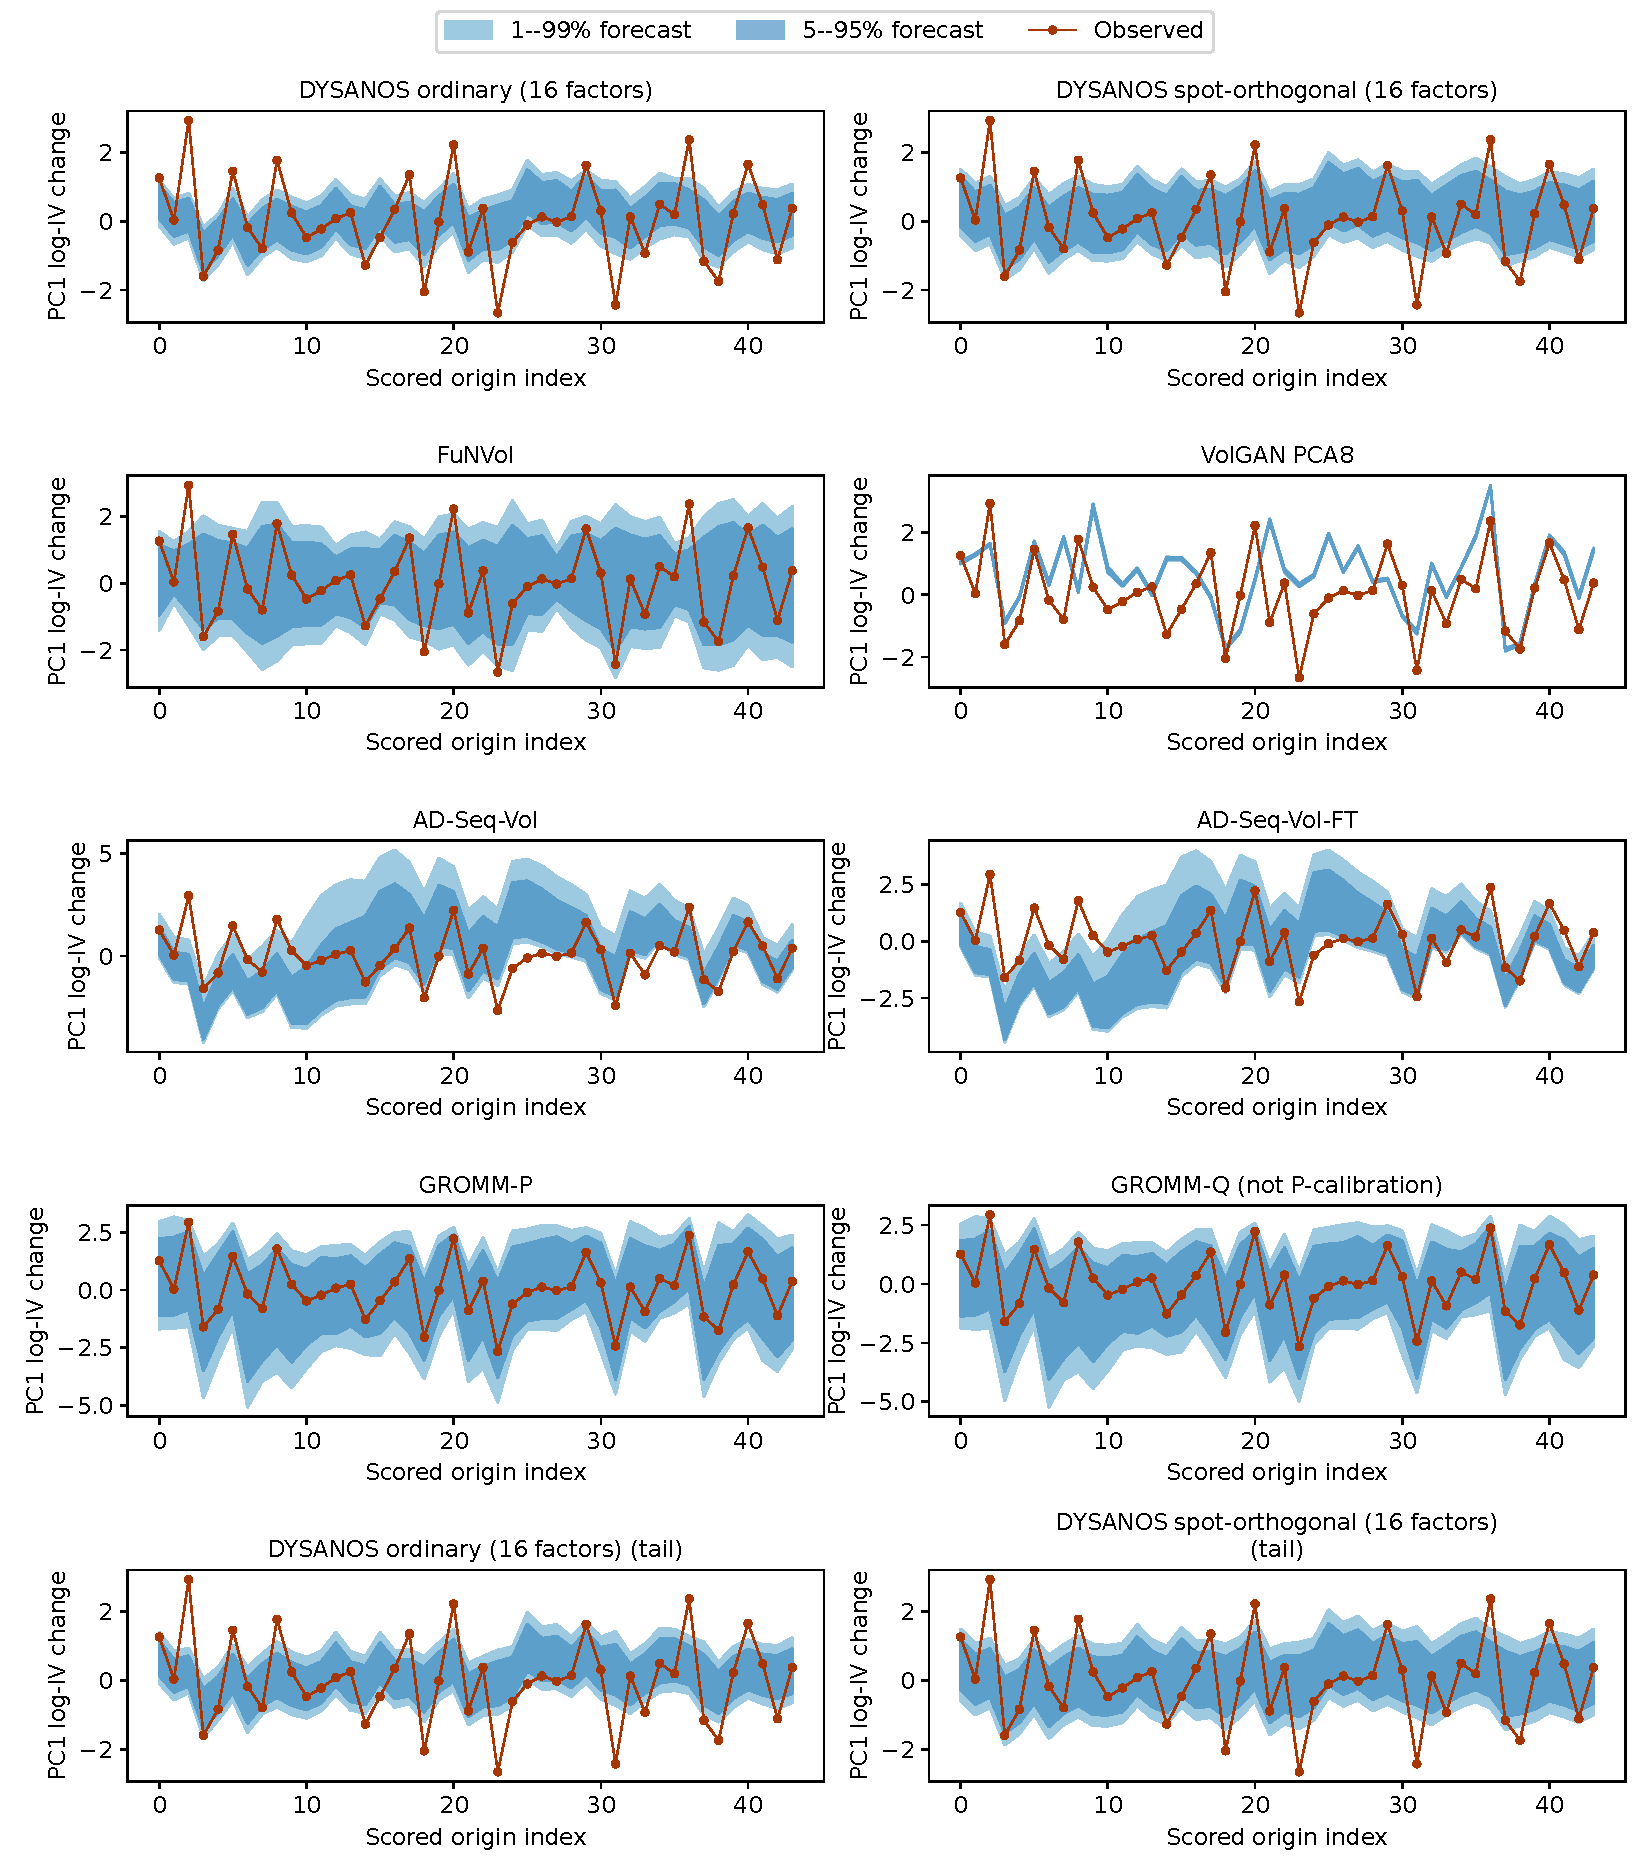
\includegraphics[width=\linewidth]{tails.pdf}\caption{Raw PC1 forecast bands and observed changes. Narrow forecast bands can reveal severe conditional underdispersion even when pooled covariance looks realistic.}\end{figure}

The lower 5\% ES estimate is the Monte Carlo mean below the empirical 5\% quantile. The JSON contains the joint Fissler--Ziegel score, with $G_1=0$, $G_2(e)=\exp(e)$, for signed lower-tail ES:

\[S_\alpha(y,q,e)=e^e\left[e-q+\frac{\mathbf1_{\{y\le q\}}}{\alpha}(q-y)-1\right].\]

Lower expected score is better for a fixed target and units. Unlike the negative-ES-only FZ0 specialization, this choice does not discard forecasts whose lower-tail ES is positive. Scores of differently scaled targets are not pooled into a headline ranking.

\section{PCA--AR(1) stationarity and floating-IV persistence}

The analytic stationarity question is restricted to the fitted floating-volatility PCA backbone, with coefficients frozen at each origin. Write its transition as

\begin{equation} h_{n+1}=b+A h_n+\varepsilon_{n+1},\qquad E[\varepsilon_{n+1}]=0,\quad\operatorname{Cov}(\varepsilon_{n+1})=Q.\end{equation}

Innovations are independent across sessions under the fitted law and have finite covariance. A Gaussian stock-return innovation may contribute to $\varepsilon$; it changes $Q$, including any stock--factor cross-covariance, not the stability criterion. No stationarity condition is imposed on the stock price. A sufficient condition for a unique causal stationary backbone, and the criterion tested here, is

\begin{equation}\rho(A)<1,\qquad \bar h=(I-A)^{-1}b,\qquad V=A V A^\top+Q.\end{equation}

The Lyapunov solution $V$ is the stationary covariance. If the complete innovation vector is jointly Gaussian, the stationary law is $N(\bar h,V)$; Gaussianity is not needed for covariance stationarity. For the orthogonal variant, the innovation covariance includes the stock loading projected onto the 16 PCA coordinates. Starting a forecast at the observed state need not start it in its invariant distribution: the stable backbone converges toward that law. This is a per-fit assessment, not a claim that a daily re-estimated sequence has constant parameters.

Let $z_{j,t}=U_j^\top x_t$. The PCA basis is fixed before April, while each model may continue using its own daily rolling factors internally. We never concatenate native factor scores across changing bases. We separately retain level ACF, change ACF and expiry-by-expiry ATM log-IV level ACF. Exact session separations are used; lag 21 has 23 observed pairs and lag 63 has none.

\begin{figure}[H]\centering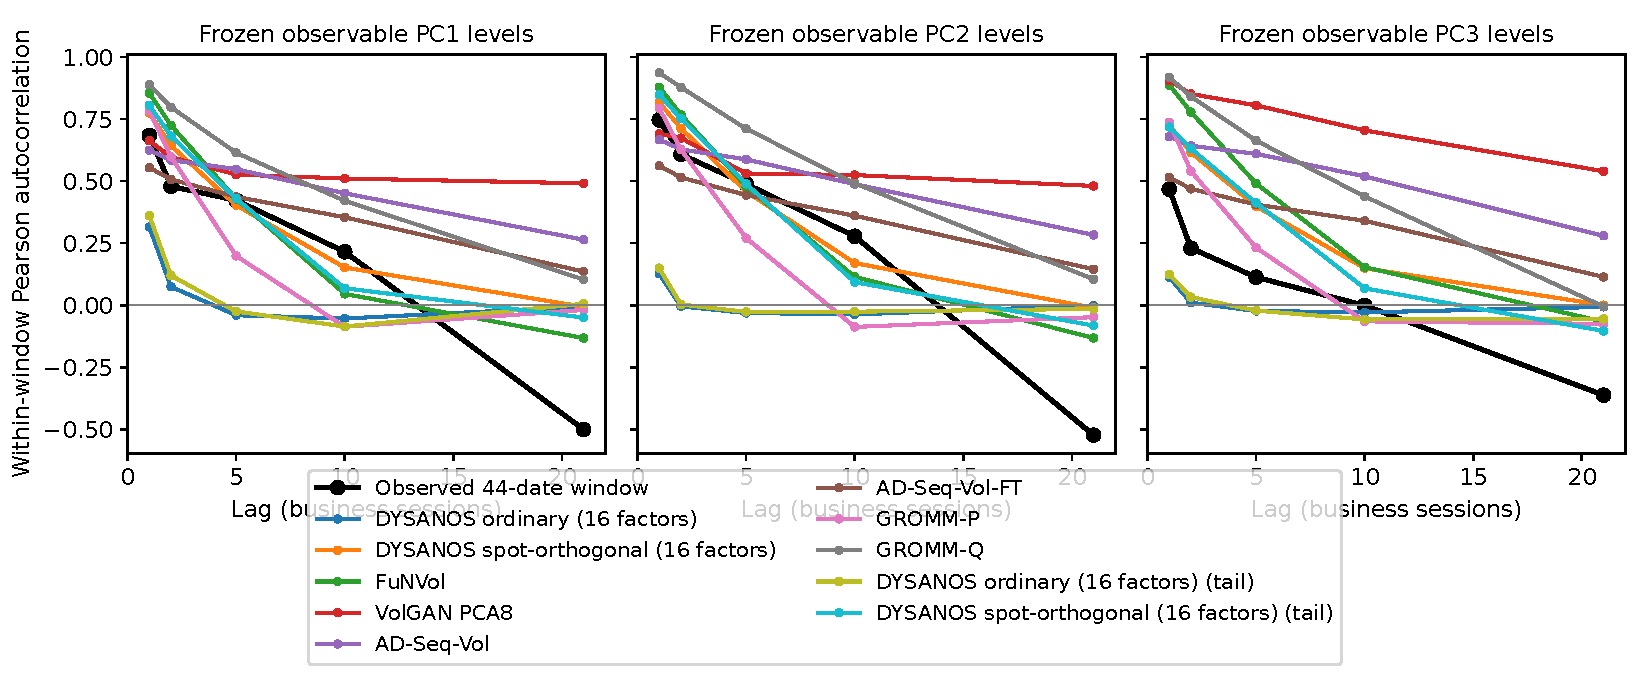
\includegraphics[width=\linewidth]{acf.pdf}\caption{PCA-level autocorrelation decay. Model curves average within-path Pearson ACFs from the first 44 simulated sessions, matching the observational window length; they are not formed by concatenating different dates' rolling models. The full 128-session checks are stored separately. Short-window detrending can itself produce negative long-lag estimates.}\end{figure}

\begin{table}[H]\centering\small\setlength{\tabcolsep}{4pt}
\caption{Maximum absolute floating-IV ACF discrepancy across the three fixed observable PCs. Lag 21 has only 23 observed pairs, so cannot receive black. Color rules: Maximum absolute PC-ACF error: black at most 0.10, orange above 0.10 through 0.20, red above 0.20. Fewer than 30 observed lag pairs forces at least orange, even for a small error. Missing graded entries are orange; other raw quantities are ungraded.}\label{tab:acf-errors}
\begin{tabular}{@{}lrrr@{}}
\toprule
Model & Lag 1 error & Lag 5 error & Lag 21 error \\
\midrule
DYSANOS ordinary (16 factors) & \textcolor{red}{0.620} & \textcolor{red}{0.519} & \textcolor{red}{0.522} \\
DYSANOS spot-orthogonal (16 factors) & \textcolor{red}{0.258} & \textcolor{red}{0.285} & \textcolor{red}{0.513} \\
FuNVol & \textcolor{red}{0.419} & \textcolor{red}{0.378} & \textcolor{red}{0.391} \\
VolGAN PCA8 & \textcolor{red}{0.437} & \textcolor{red}{0.692} & \textcolor{red}{1.004} \\
AD-Seq-Vol & \textcolor{red}{0.212} & \textcolor{red}{0.497} & \textcolor{red}{0.807} \\
AD-Seq-Vol-FT & \textcolor{orange}{0.185} & \textcolor{red}{0.293} & \textcolor{red}{0.668} \\
GROMM-P & \textcolor{red}{0.269} & \textcolor{red}{0.224} & \textcolor{red}{0.481} \\
GROMM-Q & \textcolor{red}{0.451} & \textcolor{red}{0.550} & \textcolor{red}{0.628} \\
DYSANOS ordinary (16 factors) (tail) & \textcolor{red}{0.597} & \textcolor{red}{0.515} & \textcolor{red}{0.509} \\
DYSANOS spot-orthogonal (16 factors) (tail) & \textcolor{red}{0.250} & \textcolor{red}{0.299} & \textcolor{red}{0.451} \\
\bottomrule\end{tabular}\end{table}

For DYSANOS only, we report the saved backbone spectral radius, modal damping half-lives $\log(1/2)/\log|\lambda_j|$ for stable nonzero eigenvalues, and innovation variance traces at horizons 1,5,21,63. Complex/negative eigenvalues describe oscillatory damping, not a monotone scalar half-life. Half-lives are measured in business sessions. Stationary means, covariances and numerical Lyapunov residuals are retained in the dated JSON files. All 88 fitted radii are already below one before the configured spectral-radius cap is applied.

\begin{table}[H]\centering\small\setlength{\tabcolsep}{4pt}
\caption{Stationarity of the floating-volatility PCA--AR(1) backbones; half-lives are in business sessions. Color rules: AR spectral radius: black below 0.99, orange from 0.99 to below 1, red at least 1. Stable-fit counts and half-lives are ungraded. Missing graded entries are orange; other raw quantities are ungraded.}\label{tab:ar-stationarity}
\begin{tabular}{@{}lrrrr@{}}
\toprule
DYSANOS backbone & Stable fits & Min radius & Max radius & Max half-life \\
\midrule
DYSANOS ordinary (16 factors) & 44/44 & \textcolor{black}{0.565} & \textcolor{black}{0.735} & 2.246 \\
DYSANOS spot-orthogonal (16 factors) & 44/44 & \textcolor{black}{0.574} & \textcolor{black}{0.730} & 2.201 \\
\bottomrule\end{tabular}\end{table}

The separate recursive tests below concern decoded floating IVs, not stationarity of spot and not an additional acceptance condition for the PCA--AR backbone. They retain the original model laws without substituting Gaussian stock shocks or changing fitted coefficients.

\begin{table}[H]\centering\small\setlength{\tabcolsep}{4pt}
\caption{Recursive floating-IV diagnostics: evaluated origins and extreme/invalid rates. Color rules: Extreme-surface rate (any common-grid IV above 300\%): black zero, orange above zero through 0.1\%, red above 0.1\%. Invalid-path rate: black zero, orange above zero through 1\%, red above 1\%. Evaluated-origin counts are neutral. Missing graded entries are orange; other raw quantities are ungraded.}\label{tab:recursive-stability}
\begin{tabular}{@{}lrrr@{}}
\toprule
Model & Recursive origins & Extreme surface rate & Invalid path rate \\
\midrule
DYSANOS ordinary (16 factors) & 44 & \textcolor{black}{0.000} & \textcolor{black}{0.000} \\
DYSANOS spot-orthogonal (16 factors) & 44 & \textcolor{black}{0.000} & \textcolor{orange}{0.001} \\
FuNVol & 44 & \textcolor{black}{0.000} & \textcolor{black}{0.000} \\
VolGAN PCA8 & 44 & \textcolor{red}{0.767} & \textcolor{black}{0.000} \\
AD-Seq-Vol & 44 & \textcolor{black}{0.000} & \textcolor{black}{0.000} \\
AD-Seq-Vol-FT & 44 & \textcolor{black}{0.000} & \textcolor{black}{0.000} \\
GROMM-P & 44 & \textcolor{black}{0.000} & \textcolor{black}{0.000} \\
GROMM-Q & 44 & \textcolor{black}{0.000} & \textcolor{black}{0.000} \\
DYSANOS ordinary (16 factors) (tail) & 44 & \textcolor{black}{0.000} & \textcolor{black}{0.000} \\
DYSANOS spot-orthogonal (16 factors) (tail) & 44 & \textcolor{black}{0.000} & \textcolor{black}{0.000} \\
\bottomrule\end{tabular}\end{table}

An extreme surface has at least one common-grid annual IV above 3.0 (300\%). All option-price inversion uses vectorized \texttt{cdxcore.bs.implied} on raw, unclipped inputs, with its $10^{-8}$ price tolerance and an independent vectorized \texttt{bs.price} repricing check. The former additional time-value/interiority veto has been removed. The library's default 1\%--500\% volatility bounds and intrinsic-price conventions are retained and counted explicitly; a library boundary estimate is not called a failed model path solely for having tiny time value. Native-price bound violations and repricing residuals remain recorded. These numerical point estimates do not imply uniquely identified wing volatilities at sub-tolerance prices. A completed test with no usable complete IV paths remains in coverage and invalid-rate statistics but has no ACF. All DLV clipping counts are retained separately. Recursive paths use frozen fits and their original innovation laws; finite-horizon survival is not a non-explosion proof.

\appendix\section{Model-specific implementation choices and difficulties}

This appendix is AI-agent implementation feedback based on actual retained code and artifacts, not a claim that these choices are prescribed by the cited papers. Existing model laws and fits are unchanged; the additional May FT fits use the same rolling recipe and are separately identified. The audit does not treat legacy hedging results as newly validated.

\subsection{Our DYSANOS fits: ordinary and spot-orthogonal}

Both variants use the retained nine tenors $(1,2,3,4,5,10,15,20,25)$, 200 interior strikes and native NMS $(-4,3)$. Daily source prices came from saved 0.1-SANOS surfaces; the representation itself has zero backbone smoothing. Native coordinates contain nine blocks of 200 log-DLV-squared coordinates plus a log-forward-volatility coordinate (1809 in total). This is not the later requested 13-tenor correction, and not the former 1811-coordinate smoothed SANOS state.

Each daily fit uses 252 eligible exact-session transitions, rank 16, ridge $10^{-6}$ and spectral-radius cap 0.999. Factor orientation is aligned to the preceding fit. The raw and constrained radii are both saved. The orthogonal variant first removes the spot projection from state changes and adds its loading back during simulation. The analytic stationarity score tests the 16 floating-volatility AR coordinates only; its innovation covariance includes the projected stock contribution and cross-covariances, without testing stock-price stationarity.

The legacy conversion contains zero-over-zero/unidentified and floored DLV coordinates. The report preserves their counts rather than explaining them away as successful calibration. The model decoder retains local-volatility bounds 0.001--1000 and the numerical log-strike bound 30; it records clipping. For one-day forecasts we enumerate all 252 paired empirical innovations exactly. These repeated historical shocks are not 10,000 independent observations. Spot follows the original residual bootstrap here, not a newly imposed front-density marginal. These defects and choices limit the interpretation of this legacy model.

Across the 44 origins, the mean native 16-PC variance coverage is 83.77 percent for ordinary PCA and 83.86 percent after spot orthogonalisation. The daily conversion has 296--453 floored nodes out of 1800 DLV coordinates (median 390). Native-coordinate coverage is not the same denominator as observable log-IV-change coverage.

\subsection{Additional causal Tail Diffusion cases}

Both ordinary and spot-orthogonal variants retain the same surface decoder and 16-factor AR coefficients but replace empirical surface-innovation replay by the paper's scalar log-variance OU scale mixture. Normal spot innovations are separated by the fitted joint covariance; tail scaling applies to the spot-conditioned Gaussian surface residual. Each dated tail law uses only that fit's preceding 252 exact-session innovations, resetting the latent filter across gaps. Its likelihood uses the existing Gaussian approximation to log-chi-square radius measurements, here in 16 dimensions rather than the paper's 200-dimensional application. This approximation is an explicit limitation.

With fitted conditional factor loading $L$, the surface shock is $\sqrt{\rho\exp(g-v_g/2)}Lz$, while $g^+=\phi g+\sqrt{v_g(1-\phi^2)}\xi$. The existing tail fitter estimates $(\rho,\phi,v_g)$, adding the previous origin's parameters as an optimizer start. The initial latent law is the causal one-step predictive distribution from the trailing radius filter, not an unconditional stationary reset at every simulated session. No April--May future observation tunes these parameters. One-day forecasts use 10,000 draws and recursive tests the same 32 paths over 115 sessions. Tail thickness is not artificially rescaled to match test-window variance.

At this build there are 88 tail fits and 1 raw optimizer warnings. 1 warning cases have independent projected-gradient verification at $10^{-6}$ mean-log-likelihood accuracy, without changing parameters. Exact original messages remain in the fitted records and review sidecars; a local gradient check is not a global-optimum certificate.

\subsection{FuNVol}

This is the single-asset adaptation on the seven-tenor, 19-NMS-node short-end grid. Inverse-softplus IVs are smoothed on a fourth-order Legendre basis, then reduced to three functional PCs. Joint score/log-spot dynamics use separate drift and diffusion GRUs: three layers, width 16, ten-state history, Gaussian increments over 1/252 year. The FPC basis and normalization are inherited through the rolling checkpoint chain, not recomputed daily. A 2022 comparison selected 100 rolling epochs; subsequent daily fits used all their causal window rather than a future holdout.

The first causal April fit generated spot volatility 0.333\% against trailing historical 0.778\%, failing the original 0.5-ratio dispersion gate. The user explicitly authorized proceeding with those numbers. The warning remains part of the model interpretation; no calibration pass is retroactively claimed. Softplus ensures positive IV, not absence of static/dynamic arbitrage. The earlier narrow static-arbitrage screen covered only 11 strikes within approximately 0.5\% of ATM. The present central-grid audit is different and is not an arbitrage proof.

The retained first-April FPC basis reports 97.849\% cumulative training variance coverage for its three components. This is variance of Legendre-smoothed inverse-softplus IV levels in its initializer coordinate system, not variance coverage of daily observable log-IV changes in the audit. These percentages must not be compared without their denominators.

Reference: Choudhary, Jaimungal and Bergeron, FuNVol, Quantitative Finance 24 (2024), DOI \href{https://doi.org/10.1080/14697688.2024.2396977}{10.1080/14697688.2024.2396977}.

\subsection{VolGAN PCA8}

The retained model is the paper-inspired eight-PC adaptation, not the original full-surface VolGAN. Separate train-only bases compress log-IV levels in the condition and log-IV changes in the output. Spot return remains an explicit output. Frozen initializer bases are inherited across dates; network weights and latent normalization are updated causally. Conditioning includes two previous annualized returns and trailing 21-session realized volatility. Softplus networks use noise dimension 32 and hidden dimension 16.

The 2022 initializer trained for 10,000 epochs; selected rolling updates use 300 epochs, and 10,000 sampled scenarios per origin is a different quantity. PCA bases and scaling use only training data. The gradient-matching phase continues from updated weights rather than restarting; its 25 epochs are included in the training total. The initializer selected rolling-update settings on a shorter 200-observation 2022 window because fewer than 252 observations were available. The native-model and short-end-data adaptations must not be described as an exact reproduction of published results.

The one-day surface audit re-samples the saved, version-checked checkpoints on CPU with seed 20261111, preserving the model's decoding and conditioning. Recursive sampling updates each path's own IV surface, recent returns and realized-volatility condition; it does not feed actual future market data back in. Conditional collapse and recursive extreme IVs are reported, not repaired by rescaling shocks.

Reference: Vuletic and Cont, VolGAN, DOI \href{https://doi.org/10.1080/1350486X.2025.2471317}{10.1080/1350486X.2025.2471317}.

\subsection{AD-Seq-Vol and fine-tuned AD-Seq-Vol-FT}

The short-end input is a 22-session sequence of log-IV and broadcast normalized-forward return channels; 21 sessions condition the next. The retained architecture uses a causal transformer of width 256, eight layers, four heads and a 200-step cosine diffusion. The fine-tuned variant freezes the EMA base and fits a zero-initialized rank-four output adapter with static-arbitrage penalties. Neither variant is a risk-neutral generator.

Published training settings include learning rate $7\cdot10^{-5}$, batch size 256, weight decay 0.01, 1600 warm-up steps, EMA 0.995 and a 3000-epoch initializer. Dated rolling fits warm-start from prior weights; their original normalization is kept fixed because rebasing would change the diffusion-noise law. The newest 20\% of training sequences is validation. The April base checkpoint is present but its first next-IV scenario artifact was missing; the audit regenerates 512 CPU paths in eight batches of 64 from the authenticated saved EMA, using batch seeds 20261111--20261118. This new forecast does not pretend to be the missing original 10,000-path sample. The 22 new May FT fits continue the 30 April checkpoint, freeze the original base, and train only the rank-four output adapter for the same one selected epoch per date. All new parent/base hashes and training dates are retained. Forecast and recursive-test completion are shown in Table~\ref{tab:audit-coverage}, not inferred from training completion. Recursive diffusion uses all 200 denoising steps each session and the original weekly adapter's context rule: spatially average the generated return channel and rebroadcast that scalar when appending each path's own next state. Per-session checkpoints retain context, generated IVs and RNG state.

Reference: Han, Zhang, Torres, Acero and Xu, Diffusion Models for Dynamic Volatility Surface Generation and Data-Driven Hedging, \href{https://arxiv.org/abs/2609.13402}{arXiv:2609.13402}.

\subsection{GROMM under P and Q}

P and Q share the same 44 dated affine-200 fits and rank-16 dynamics; they are not separately duplicated trained models. The retained native grid uses 200 interior strikes, NMS $(-3,2)$ and a changing union of reference/quoted expiries, not the proposed new $(-4,3)$ grid. The Black background annual volatility is 5\%. Affine fitting uses 2000 epochs, learning rate 0.01 and DLV-squared bounds $10^{-4}$--9. The original fit target is the released SANOS price panel with stored half-spreads, not observed midpoints. Stored training-window fit rates are therefore kept distinct from the direct licensed-quote measurements in this audit.

The retained artifacts were migrated by exact input/geometry reuse between public manifests; their source/target fingerprints and hashes remain in each dated manifest. Some migrated fits have no affine optimizer checkpoint or warm-start date. We do not silently claim they were sequentially retrained. P uses the accepted attainable physical risk-price projection; Q omits that Brownian drift shift. Both use eight Brownian DLV substeps and the original numerical scheme, including its numerical safeguards. An AR-related physical drift estimate is not a global linear VAR transition for the decoded risk-neutral surface; spectral radius is therefore n/a.

The stored native explained-variance ratio of 1.0 on the first fit uses Gaussian-smoothed, centered native log-DLV innovations restricted to the fitted strike core, including the spot projection plus residual factors. It is not 100\% coverage of raw full-grid IV changes or an out-of-sample claim. This report instead measures all models directly in the same observable space.

The new observable audit generates 512 antithetic paths (256 shock pairs) per date and measure with seed 20261111 on CPU, using the saved fits without training. It prices the native density tower plus background factor and converts to floating common-grid IVs. Terminal tenors are aged correctly: tomorrow's 1D row comes from today's 2D expiry. This differs from the retained 10,000-path price-return books used for the quoted-book forecast audit. Monte Carlo uncertainty of 512 paths and 44 realized dates must not be conflated. Common random seeds across origins are intentional, not additional independent market observations. Q-versus-P empirical comparisons are explicitly labelled descriptive.

The retained GROMM integrator tames an Euler relative-drift increment $x$ only when $|x|>0.5$, replacing it with $\operatorname{sgn}(x)[0.5+\log(1+|x|-0.5)]$ before the exponential variance update. This is an implementation stabilization, not the unchanged continuous-time drift restriction and not a proof of exact finite-step martingality. Taming frequency was not retained in the new observable extracts, so no zero-intervention claim is made. Float32 saved density inputs are decoded in float64 and normalized only within the source-precision mass-error tolerance; the diagnostic logs preserve the errors and tolerances.

\subsection{Hedge wrappers and non-generative baselines}

Greek, parametric and statistical hedge wrappers do not constitute three separately trained surface generators when they reuse the same DYSANOS state and dynamics. Their underlying-law diagnostics are shared. Unhedged, Black delta and Black delta-plus-vega are hedging baselines, not joint stochastic IV-surface models, so covariance, PCA persistence and linear-core spectral radius are not fabricated for them. No hedge objective, risk aversion, transaction-cost setting or optimizer was changed or rerun by this audit.

\subsection{Inference-only model retention}

At the user's request, the diffusion models now have an EMA-only inference archive with exact content-addressed backbone sharing. 88 dated exports have been checked tensor by tensor and through two seeded complete 200-step CPU sampling paths against their original checkpoints, with zero differences. Geometry, versions, normalization, dated adapters and historical source hashes are retained. 88 redundant restart checkpoints (4.430 GiB gross) have been retired; the inference archive occupies 0.756 GiB. This preserves inference, not exact optimizer/RNG restart. Original fitted laws are unchanged; inference operability is not a calibration-quality pass. Other models, historical contexts, retained scenarios and results have not been deleted by this step.

\section{Reproducibility and missing evidence}

Licensed data and fitted parameters are unchanged. Large models, retained scenario arrays and licensed quote rows remain external; only aggregates, diagnostics and checksummed manifests are suitable for Git. Retired checkpoint identities resolve through \path{INFERENCE_MODELS.json}; \path{model_audit/inference.py} loads the verified inference replacements without optimizer or training data.

The report is generated by \path{quantdata/hedging/model_audit/report.py}; \path{run.py}, \path{persistence.py}, \path{gromm.py} and \path{quotes.py} reproduce its stages. Interpreter: \path{/home/hans/vqdata/bin/python}. Jobs set explicit \texttt{QUANTDATA\_ROOT} and \texttt{PYTHONPATH}. Neural recursive paths use a managed GPU; other audit stages run on CPU. Disjoint origin batches preserve each origin's seed, saved context and RNG state. No diffusion denoising steps are dropped.

The JSON daily files retain failure reasons, no-data exclusions, quantile forecasts, full conditional covariance and source diagnostics. CSVs provide coverage, daily/monthly/rolling errors, per-expiry/NMS log-IV RMSE, tail tests and linear-core stability. Raw modeled means are retained: this is a model-law audit, not the demeaned hedge-optimization experiment. The 44-day report cannot establish 63-day observed ACF or reliable 1\% tail calibration. Missing diagnostics remain n/a.

\end{document}
